
\section{Juegos Serios}
\setcounter{sectiontotal}{5}

\begin{frame}
    \frametitle{\pagetitle}
    \framesubtitle{Definición}
    \begin{block}{Juego Serio}
    \centering
    Es un juego que posee un propósito educacional explícito, cuyo objetivo
    principal es el de educar y utiliza conceptos lúdicos para involucrar y
    entretener al usuario
    \end{block}   
    \begin{center}
    
\includegraphics[scale=.5]{imagenes/juegos_educacion}
    \end{center}
\end{frame}

\begin{frame}
    \frametitle{\pagetitle}
    \framesubtitle{Características}
    \begin{columns}
    \column{.7\textwidth} \hspace{0.5cm}
     \begin{itemize}[<+->]
         \item Contexto.
         \item Construcción.
         \item Relación con profesionales de la educación.
         \item Nivel cognitivo del alumno.
    \end{itemize}
    \column{.4\textwidth} \hspace{0.5cm}
    
\includegraphics[scale=0.25]{imagenes/aprendizaje}
    \end{columns}
\end{frame}

\begin{frame}
\frametitle{\pagetitle}
\framesubtitle{Ventajas}

\begin{itemize}[<+->]
    \item Motivación interna\sfcite{guenaga2013serious}.
    \item Apoyo al aprendizaje\sfcite{sg:aoverview}.
    \item Menos limitaciones\sfcite{sg:aoverview}.
    \item Similitud a la realidad\sfcite{sg:aoverview}.
    \item Estimulación sensorial\sfcite{guenaga2013serious}.
\end{itemize}


\end{frame}
\note{Mencionar ventajas de las TIC}

\begin{frame}
    \frametitle{\pagetitle}
    \framesubtitle{Desafíos}
	\begin{itemize}[<+->]
        \item Falta de investigación\sfcite{sg:aoverview}.
        \item Expectativas muy altas\sfcite{education:games}.
        \item Evaluación tradicional\sfcite{shute2009melding}.
        \item Utilización incorrecta\sfcite{stapleton2004serious}.
        \item Falta de recursos\sfcite{sg:aoverview}.
    \end{itemize}
\end{frame}

\begin{frame}
\frametitle{\pagetitle}
\framesubtitle{Áreas de aplicación}

\pause{}
\begin{columns}
\column{.7\textwidth} \hspace{0.5cm}
\begin{itemize}[<+->]
	 \item Militar
     \item Salud
     \item Juegos corporativos
\end{itemize}

\column{.4\textwidth} \hspace{0.5cm}
\begin{overprint}
    \onslide<2|handout:1> 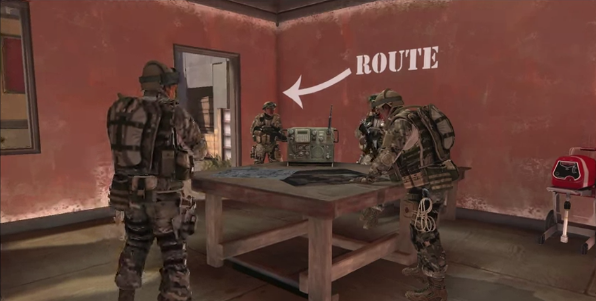
\includegraphics[width=\textwidth, height=4cm]{../tics/images/army} 
    \onslide<3|handout:0> 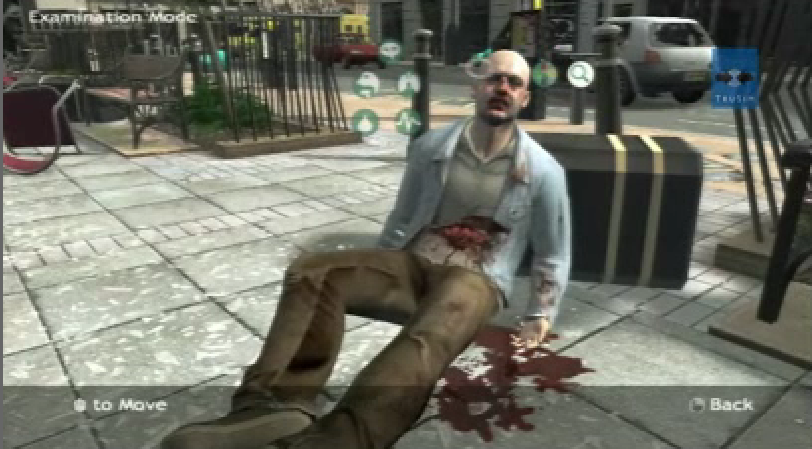
\includegraphics[width=\textwidth, height=4cm]{../tics/images/patient} 
    \onslide<4|handout:0> 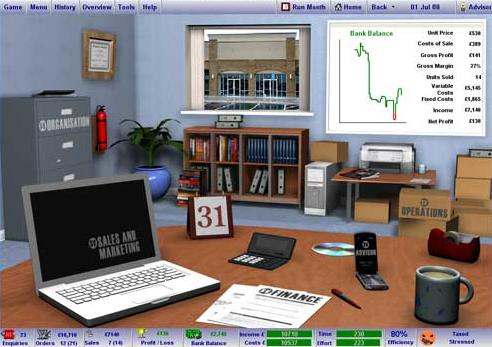
\includegraphics[width=\textwidth, height=4cm]{../tics/images/simventure} 
    
\end{overprint}

\end{columns}


\end{frame}
